\documentclass{article}
\usepackage{graphicx}
\title{Simple Regression Analysis}

\author{Stacy J Chang}

\date{October 7th, 2016}

\usepackage{Sweave}
\begin{document}
\Sconcordance{concordance:lab9.tex:lab9.Rnw:%
1 8 1 1 0 106 1}

\maketitle

\section{Abstract}

Fall 2016 Statistics 159, Reproducible and Collaborative Statistical Data Science, homework two introduced simple regrssion analysis. In this report, I utilized the Advertising CSV file that was provided to reproduce the results displayed in chapter 3, \emph{Simple Linear Regression}, of the text book, \textbf{An Introduction to Statistical Learning}. 

\section{Introduction}

The overarching goal of this homework is for the students to get familiarized with linear regression, a simple yet powerful tool to analysize data. Even though there is multiple regression analysis, this report primaryly uses simple linear regression, which only considers two variables. The report focuses on the potential relationship or regression between \textbf{Sales} and \textbf{Advertisment} in three different media outlets. 

\section{Data}

The Advertising data that used in this report was provided through the textbook, \textbf{An Introduction to Statistical Learning} written by Gareth James, Daniela Witten, Trevor Hastie and Robert Tibshirani. 

\section{Methodology}

\emph{Simple linear regression} is a very simple approach for estimating a quantitative response $Y$ on an independent variable $X$. The regression assumes that there is a linear relationship between $Y$ and $X$. The regression is usually model after this simple equation.

\begin{equation}
Y_i \approx {\beta}_0 + {\beta}_1 X_i
\end{equation}

\subsection{Estimating the Coefficients}

In this paper, we concentrated on one particular media platform, which is TV, and its relationship with **Sales**. The linear model that the we perform the simple linear regression on is:

\begin{equation}
Sales \approx \hat{\beta}_0 + \hat{\beta}_1 TV
\end{equation}

In order to accurately estimate $\hat{\beta}_0$ and $\hat{\beta}_1$ that fit our linear model, we needed to use the 200 samples that are given in the data. Ultimately, our goal is to fine the closeness between $\hat{\beta}_0$ and $\hat{\beta}_1$ and n = 200 different markets. We have to find an intercept of $\hat{\beta}_0$ and a slope $\hat{\beta}_1$ such that the resulting line is as close to the n = 200 data points. 

We used $\emph{residual sum of squares}$ (RSS) to estimate the least squares fit for the regression. Let $\hat{Y}_i = \hat{\beta}_0 + \hat{\beta}_1 X_i$ be the prediction of $Y$, and the ith residuals is $e_i = y_i - y_i$. $\emph{Residual sum of squares}$ (RSS) is:

\begin{equation}
RSS = e_1^2 + e_2^2 + \cdots + e_3^2
\end{equation}

Utilizing this knowledge, we found that $\hat{\beta}_0 = 7.03 and \hat{\beta}_1 = 0.0.475$. These values translate to that with an additional of \$1000 spent on TV advertisement is associated with selling approximately 47.5 additional units of product. 

\subsection{Assesing the Accuracy of the Coefficients Estimates}

The observed $\beta$ values can be used to come up with a hypothesis test on whether or not there is a relationship between $X$ and $Y$. Our null hypothesis would be that there is no relationship between the two variables and we perform a \emph{t-test} in order to test the hypothesis:

\begin{equation}
t = \hat{\beta_1} - 0 / SE(\beta_1)
\end{equation}

The result of the above equation is the p-value. With a small p-value, typically less than 0.05, we would be able to reject our nulll hypothesis and conclude that there is a relationship between the two variables.

\subsection{RSE}

RSE or \emph{residual standard error} estimates the standard error or the given model. The equation for it is:

\begin{equation}
\sqrt( 1/ (n-2) * \sum_{i=1}^n (y_i - yhat_i)^2)
\end{equation}

\subsection{$R^2$}

$R^2$ value measures how close the data are to the fitted regression line. The value of $R^2$ lies between zero and one. The equation of $R^2$ is:

\begin{equation}
R^2 = (TSS - RSS) / TSS
\end{equation}

\section{Results}

The result that we obtain for $\hat{\beta}_0$ and $\hat{\beta}_1$ is described in the below table:

\begin{tabular}{|l|r|r|r|r|} \hline
\bf         & Estimate & Std. Error & t value & P-value  \\\hline
(Intercept) & 7.03     & 0.46       & 15.36   & < 0.0001 \\
TV          & 0.05     & 0.00       & 17.67   & < 0.0001 \\\hline
\end{tabular}

Table: Information about Regression Coefficients

As one can see, the p-values are all less than 0.0001, which means that we can reject the null hypothesis, in other words, there is a relationship between $X$ and 
$Y$.

The table below describes additional information about the least squares model for the regression:

\begin{tabular}{|l|r|} \hline
\bf Quantity  & Value  \\\hline
    RSE       & 3.26   \\
    $R^2$     & 0.61   \\
    F-stat    & 312.14 \\\hline
\end{tabular}

Table: Regression Quality Indices

The RSE value is about 3.26, which means that on average actual sales in each market deviate from the true regression line by approximately 3,260 units. 

Below is the scatterplot showing the relationship between \textbf{Sales} and \textbf{TV}:

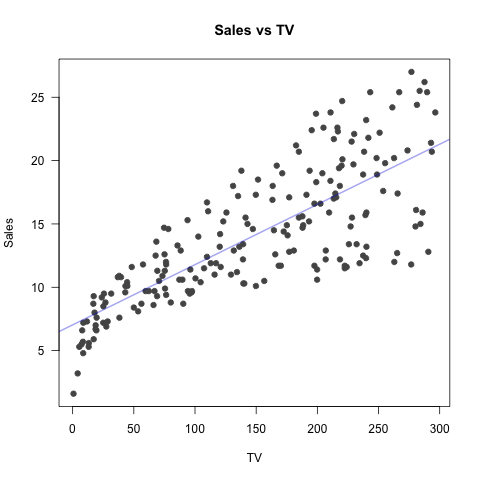
\includegraphics{images/scatterplot}

As one can see the positive slope of the regression line placed in the center of the data points, which means there is a positive correlation with the two variables.  

\section{Conclusions}

In conclusion, using simple linear regression model we found the relationship between \textbf{Sales} and \textbf{TV} advertisement. We conclude that approximately with an increase of \$1000 spendingi in TV advertisment is equalvilant as selling approximately 47.5 units of product. With an relatively easy linear regression model, we were able to predict and estimate powerful data that are essential to successfully analysize the data. The linear regression relationship between $X$ and $Y$ variables is the key aspect to the paper. 

\end{document}
